\documentclass{report}

\usepackage{geometry}	% Для последующего задания полей
\geometry{a4paper,top=2cm,bottom=2cm,left=2.5cm,right=1cm}

%%% Использовать другой интервал %%%
\renewcommand{\baselinestretch}{1.25}

\usepackage[english]{babel}	% Языки: русский, английский

%%% Математические пакеты %%%
\usepackage{amsmath}
%\usepackage{amsthm,amsfonts,amsmath,amssymb,amscd} % Математические дополнения от AMS

%%% Оформление абзацев %%%
\usepackage{indentfirst} % Красная строка

%%% Цвета %%%
\usepackage[usenames]{color}
\usepackage{color}
\usepackage{colortbl}

%%% Таблицы %%%
\usepackage{longtable}					% Длинные таблицы
\usepackage{multirow,makecell,array}	% Улучшенное форматирование таблиц

%%% Общее форматирование
% Корректируем подписи
\RequirePackage{caption}
\DeclareCaptionLabelSeparator{defffis}{ -- }
\captionsetup{justification=centering,labelsep=defffis}
\usepackage{soul}	% Поддержка переносоустойчивых подчёркиваний и зачёркиваний

%%% Библиография %%%
%\usepackage{cite} 	% Красивые ссылки на литературу
%\usepackage[square, numbers]{natbib} % also change to ugost2008n in styles.tex
\usepackage[square]{natbib}

%%% Изображения %%%
\usepackage{graphicx} % Подключаем пакет работы с графикой


%%% Tries harder figure positioning \begin{figure}[H] %%%
\usepackage{float}

%%%% allows to con­vert eps images to pdf for use with pdfla­tex
\usepackage{epstopdf}

%%% Гиперссылки %%%
\usepackage[linktocpage=true,
			plainpages=false,
			pdfpagelabels=false,
        	colorlinks=true]{hyperref}



\begin{document}

SUNGLINT IMAGERY FOR INVESTIGATING OCEANIC INTERNAL WAVES

\section{Abstract}

A method for retrieval of the spatial variations of the sea surface mean square slope (MSS) in sunglint imagery is applied for analysis of surface signatures of the internal waves. It is shown that internal waves are well visible via modulations of the sea surface MSS, enhancement/suppression of the MSS takes place in the zones of IW-induced surface current convergence/divergence. The results clearly demonstrate a highly feasible approach for investigation of the Ocean internal waves surface signatures.


\section{Introduction}

It is a well-known fact that the surface manifestation of the ocean dynamics (current features, eddies, fronts, internal waves etc.) can effectively be detected by spaceborne synthetic aperture radar (SAR). SAR signatures of current features result from wave-current interaction which leads to modulation of short wind waves scattering radio waves. On the other hand there are many scanners in the space operating in the visible range that could also be potentially used for investigation of ocean surface phenomena through the sea surface roughness modulations.

Recently, a new approach has been proposed to exploit the sunglint signatures of different ocean phenomena in terms of variations of the sea surface roughness mean square slope (MSS) \citep{Kudryavtsev2012a}. The developed method is applied to MODIS and MERIS sunglint imagery of internal waves (IWs). 

The main goal of the present study is to demonstrate the possibilities of satellite SAR and optical synergistic observations of the IWs, as well as to quantitatively interpret IWs signatures using radar imaging model (RIM) suggested by \cite{Kudryavtsev2005} and \cite{Johannessen2005}.


\section{Methodology and approach}

The algorithm for the sea surface MSS retrieval was first suggested by Myasoedov et al. in \cite{Myasoedov2010a} and further developed by the authors in \citep{Kudryavtsev2012a} and \citep{Kudryavtsev2012b}. The method is based on the idea that sunglint brightness depends on statistical properties of the sea surface slopes, - its MSS, skewness, peakedness etc. Cox and Munk \cite{Cox1954} derived these parameters from analysis of the sunglint shape, i.e. the derived parameters are were averaged over the sunglint width. The algorithm suggested in \citep{Kudryavtsev2012a} is focused on retrieval of ``small-scale'' (on scales which are much smaller than the sunglint width) MSS variations $\tilde{s^2}$ from the sunglint brightness variations $\tilde{B}$. The advantage of the algorithm is that it does not require an \textit{a priori} speculations about the PDF model, and the transfer function (relating brightness variations to MSS one) is found from the mean brightness field where the ``real'' PDF is explicitly built in.


\section{Study area and data}

The study is focused on optical MODIS and synthetic aperture radar (SAR) ASAR imagery around the coastal area of the North-East shelf of South America. The western equatorial Atlantic region facing the mouth of the Amazon River is an area with very complex ocean dynamics \citep{Silva2010}, in addition forced by Trade Winds \citep{Augustinus2004} plays an important role in the inter-hemispheric salt, heat and mass transfer \citep{Dengler2004, Schmitz1993}. Moreover the region is characterized by strong tidal currents \citep{Oltman1968, RockwellGeyer1996, LeBars2010} and regular occurrences of very intensive solitary and trains of internal waves (IWs) generated by semidiurnal tide \citep{Burdyugov1987, Ivanov1993}. Early field campaigns targeting IWs and their impact on wind waves breaking in this area were reported by Dulov et al. \cite{Dulov1986}  and Burdyugov et al. \cite{Burdyugov1987}. They found that during the peak generation, ``amplitude'' of the solitary IWs was about 100\textit{m}, and that passage of the IW (travelling to the N-E direction, opposite to the wind) caused strong impact on the wind wave breaking.  Occurrences of breaking waves were strongly enhanced (several times relative to the background value) when the thermocline was deepening, and significantly suppressed (almost disappearing) when the thermocline was rising. Such wave breaking enhancement/suppression has strong correlation with convergence/divergence of the currents induced by the IW on the surface.

The MODIS/Aqua image of this area in red channel (850\textit{nm}) on April 26, 2009, 16:20 is shown in Figure~\ref{fig:1} (upper left plot). Clouds mask the full view of the surface. However, the sunglint with linear brightness features inside (which may be treated as the surface signatures of the IWs) are easily recognized.


\section{Image analysis}

The image was processed with use of the algorithm described in \citep{Kudryavtsev2012a}. Field of the brightness variations  are shown in Figure~\ref{fig:1} (upper right plot). The initial image possesses the main features of the sunglint, while the brightness variations apparently contain sunglint signatures of the IWs.

The transfer function (eq. (5) in \citep{Kudryavtsev2012a}) calculated for the smooth brightness is shown in the lower left plot of Figure~\ref{fig:1}. In this case, the transfer function has no zone of the contrasts inversion appearing negative over the entire observed area. Thus the sign of the brightness contrasts are opposite to the sign of the MSS anomalies.

The MSS contrasts retrieved from the smoothed brightness fields determined from eq. (5) in \citep{Kudryavtsev2012a} is presented in Figure~\ref{fig:1} (lower right) using the transfer function shown in Figure~\ref{fig:1} (lower left). The MSS contrasts exhibit a variety of IW patterns. In particular a series of northeastward oriented IWs is revealed with a separation  distance between the leading solitons of about 130-150\textit{km}. In addition trains of IWs with wavelengths 1\textit{km} and 10\textit{km} trails behind the solitons. Since IWs in this area are assumed generated by semidiurnal tide, the phase speed of the IWs is about 3.5\textit{m/s}.   

The profiles of the MSS variations along the cross-sections A-B (marked in Figure~\ref{fig:1}) are presented in Figure~\ref{fig:2} (upper plot).  This confirms the abundance of surface signature of IWs. The manifestation of the IW solitons in MSS has a ``bi-polar'' shape consisting of negative and positive MSS anomalies. Recalling the shape of the IW soliton, we may conclude that increase of the MSS takes place in the zone of IW-induced surface current convergence (above forward slope of the solitons) and corresponding decrease in the zone of the current divergence (above the back slope of the solitons). The MSS contrast patterns induced by these IWs appear similar to the manifestation of solitary IW in wave breaking, as reported by Dulov et al. \cite{Dulov1986} in this area.


\section{Model simulations}

In order to examine if these observed IW-induced modulations of the MSS corresponds to the ``real'' one,  a model simulation was conducted using the radar imaging model (RIM) developed by \cite{Kudryavtsev2005}. The RIM model has been extensively validated against available data of radar signature of IW, and has demonstrated its validity.  As a first guess we assumed that the observed increase/decrease in the MSS takes place in the convergence/divergence of the surface currents induced by IW (i.e. $K_s \equiv \tilde{s^2} / s_0^2 \propto \partial u / \partial x$ where $K_s$ is the contrast of the MSS). The proportionality ``constant'' in this relation is a function (with dimension of time) depending on at least the wind speed and its direction, the IW characteristics (IW length, phase velocity) and the wind waves age. Nevertheless, for the given condition it may be assigned as a tuning constant $c_u$, which have to be determined after comparison of observed MSS with model simulations.  Then the surface velocity can be expressed as

\begin{equation}
u(x) = c_u \int_0^x \left( K_s - \left\langle K_s \right\rangle \right) dx
\label{eq:1}
\end{equation}

\noindent where $\left\langle K_s \right\rangle$ is ``low frequency'' oscillations in the MSS which are not visible in the data (Figure~\ref{fig:2}), but may results in artificial contribution to $u(x)$ due to cumulative integration in the equation.  These oscillations can for instance be caused by wind speed variability, and in our simulations they are removed by fitting the 3${}^{rd}$ order polynomial to the MSS data.  

The surface velocity (in eq. \eqref{eq:1}) was specified as the input parameter for RIM simulations of surface signatures of IW travelling opposite to the wind with phase velocity of  for a wind speed of 7\textit{m/s}. In these calculations the tuning constant $c_u$ in eq. \eqref{eq:1} was chosen to fit peaks of the model MSS variations associated with effect of the solitary IW to the observed one. The simulated MSS contrasts are shown in Figure~\ref{fig:2}, (upper plot) by the dashed line. Note that in order to get the right spatial location of the MSS peaks induced by solitary IWs, the model curve was shifted on 1\textit{km} to the right (towards IW direction). All in all the simulated contrasts of the IWs as manifestated in the MSS are very similar to the observed modulations. This suggests that the observed MSS modulations are indeed governed by convergence and divergence of the surface current.

The reconstructed surface velocity profile as well as the oscillations of the thermocline depth $h(x)$ are shown in Figure~\ref{fig:2} (lower plot). The latter was determined from the relation between the surface velocity and the thermocline depth (within the frame of 2-layer density model with the shallow upper and the deep lower layers) expressed as $u/c = \left( h-h_0 \right) / h $, where $h_0$ is the undisturbed depth, and $c$ is the IW phase velocity equal in our case to $c=3.5m/s$. The magnitude of the surface velocity oscillations and the thermocline depth displacement are consistent with field observations in this area as reported by \cite{Dulov1986} with amplitudes about 100\textit{m}. Assuming that $h_0 = 100m$ in our simulations, the amplitudes $h-h_0$ of the two leading solitons in Figure~\ref{fig:2} are 120\textit{m} and 80\textit{m}. This is in good agreement with \citep{Dulov1986}. This support the conclusion that MSS contrasts detected in the sun glitter are resulting from the surface roughness anomalies triggered by IW induced surface current convergence and divergence. As such it offers a very important complement to quantitative SAR interpretations of IWs.


\section{Conclusions}

An algorithm for the retrieval of the spatial variations of the MSS in sunglint imagery has been applied for analysis of the sunglint signatures of internal waves. We have found that the surface manifestation of IW waves are well visible in modulations of the sea surface slopes. Analysis of IW surface signatures in the MSS showed that the amplitude of the MSS contrasts (defined as amplitude of MSS variations scaled by mean MSS) is approximately proportional to the parameter of non-linearity of IW, i.e. proportional to the ratio of the amplitude of the surface current velocity induced by the IW to its phase velocity. Contrast enhancements of the MSS takes place in the zone of IW current convergence while suppressions are found in the divergence zones. This link between MSS anomalies and IW surface current divergence is similar to modulations of wind waves breaking by IW as observed by \cite{Dulov1986} in the same area. However, we notice that at the same choice of parameters of IW non-linearity, the measured contrasts of wave breaking were stronger by factor of five than presented here for the MSS contrasts.

Nevertheless the method clearly suggests an additional opportunity for investigation of surface signature of ocean features, including mesoscale ocean current fronts, eddies and IWs. Synergistic analysis of the MSS (derived from optical sensors) and SAR surface signatures will therefore lead to better quantitative understanding of the dynamics and wave-current interactions that dominate the manifestation of such features.


\section{Acknowledgments}

Core support for this study was provided by Mega-grant of the Russian Federation Government to support scientific research under the supervision of leading scientist at RSHU, No. 11.G34.31.0078.

\bibliographystyle{./agufull08}
\bibliography{./myasoedov_grl2013}

\begin{figure}
\noindent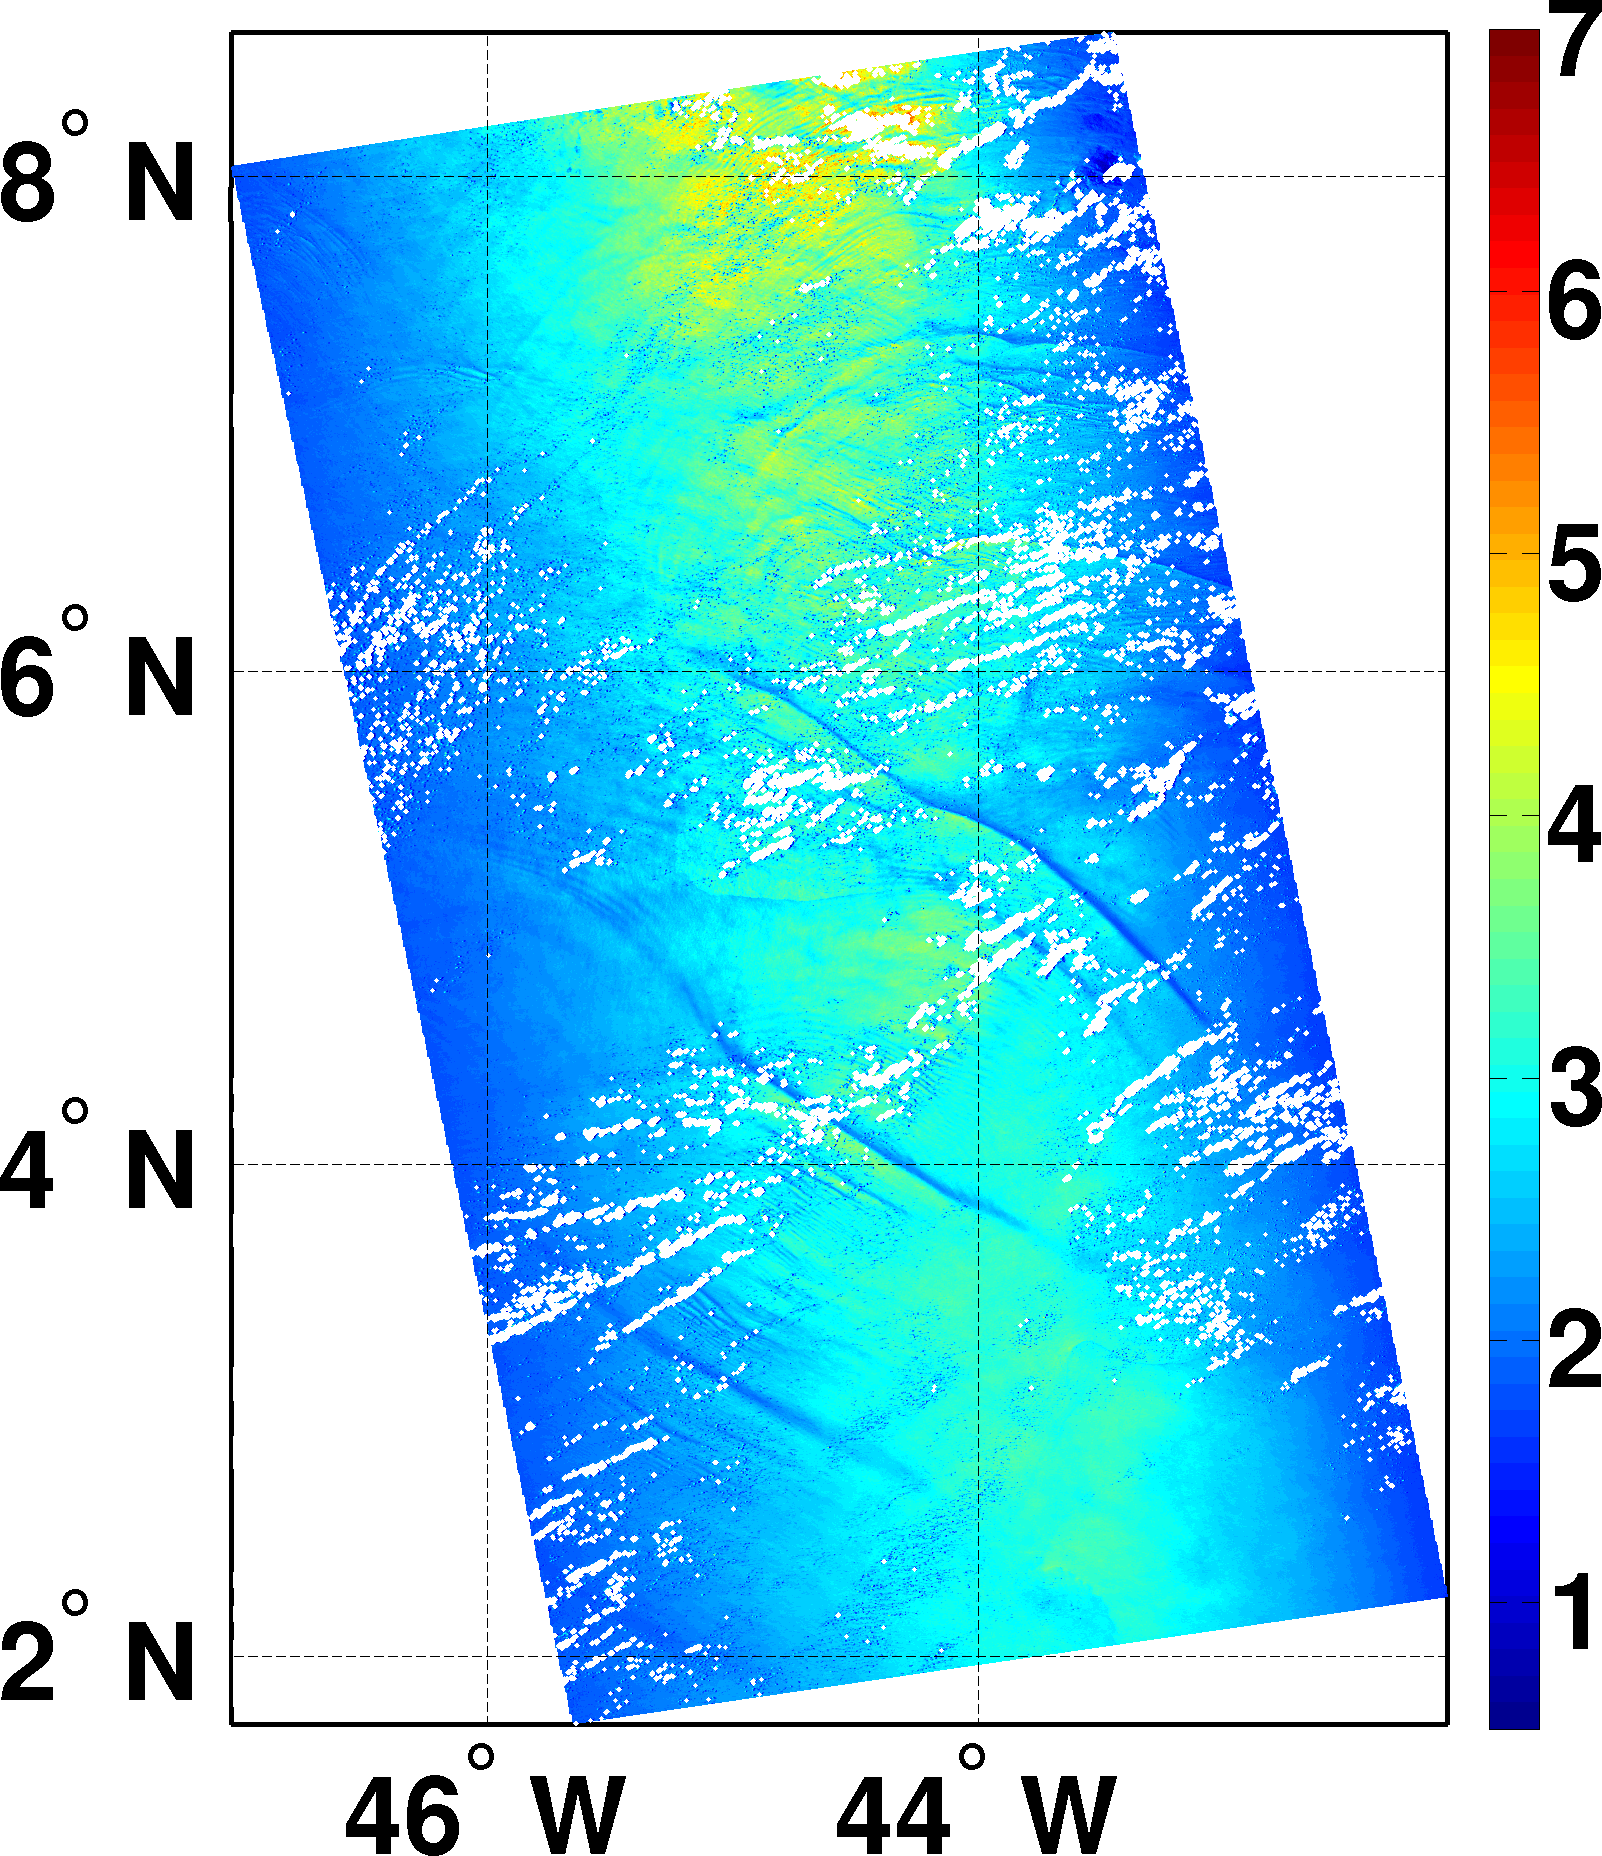
\includegraphics[width=18.5pc]{fig1a}
\hfill
\noindent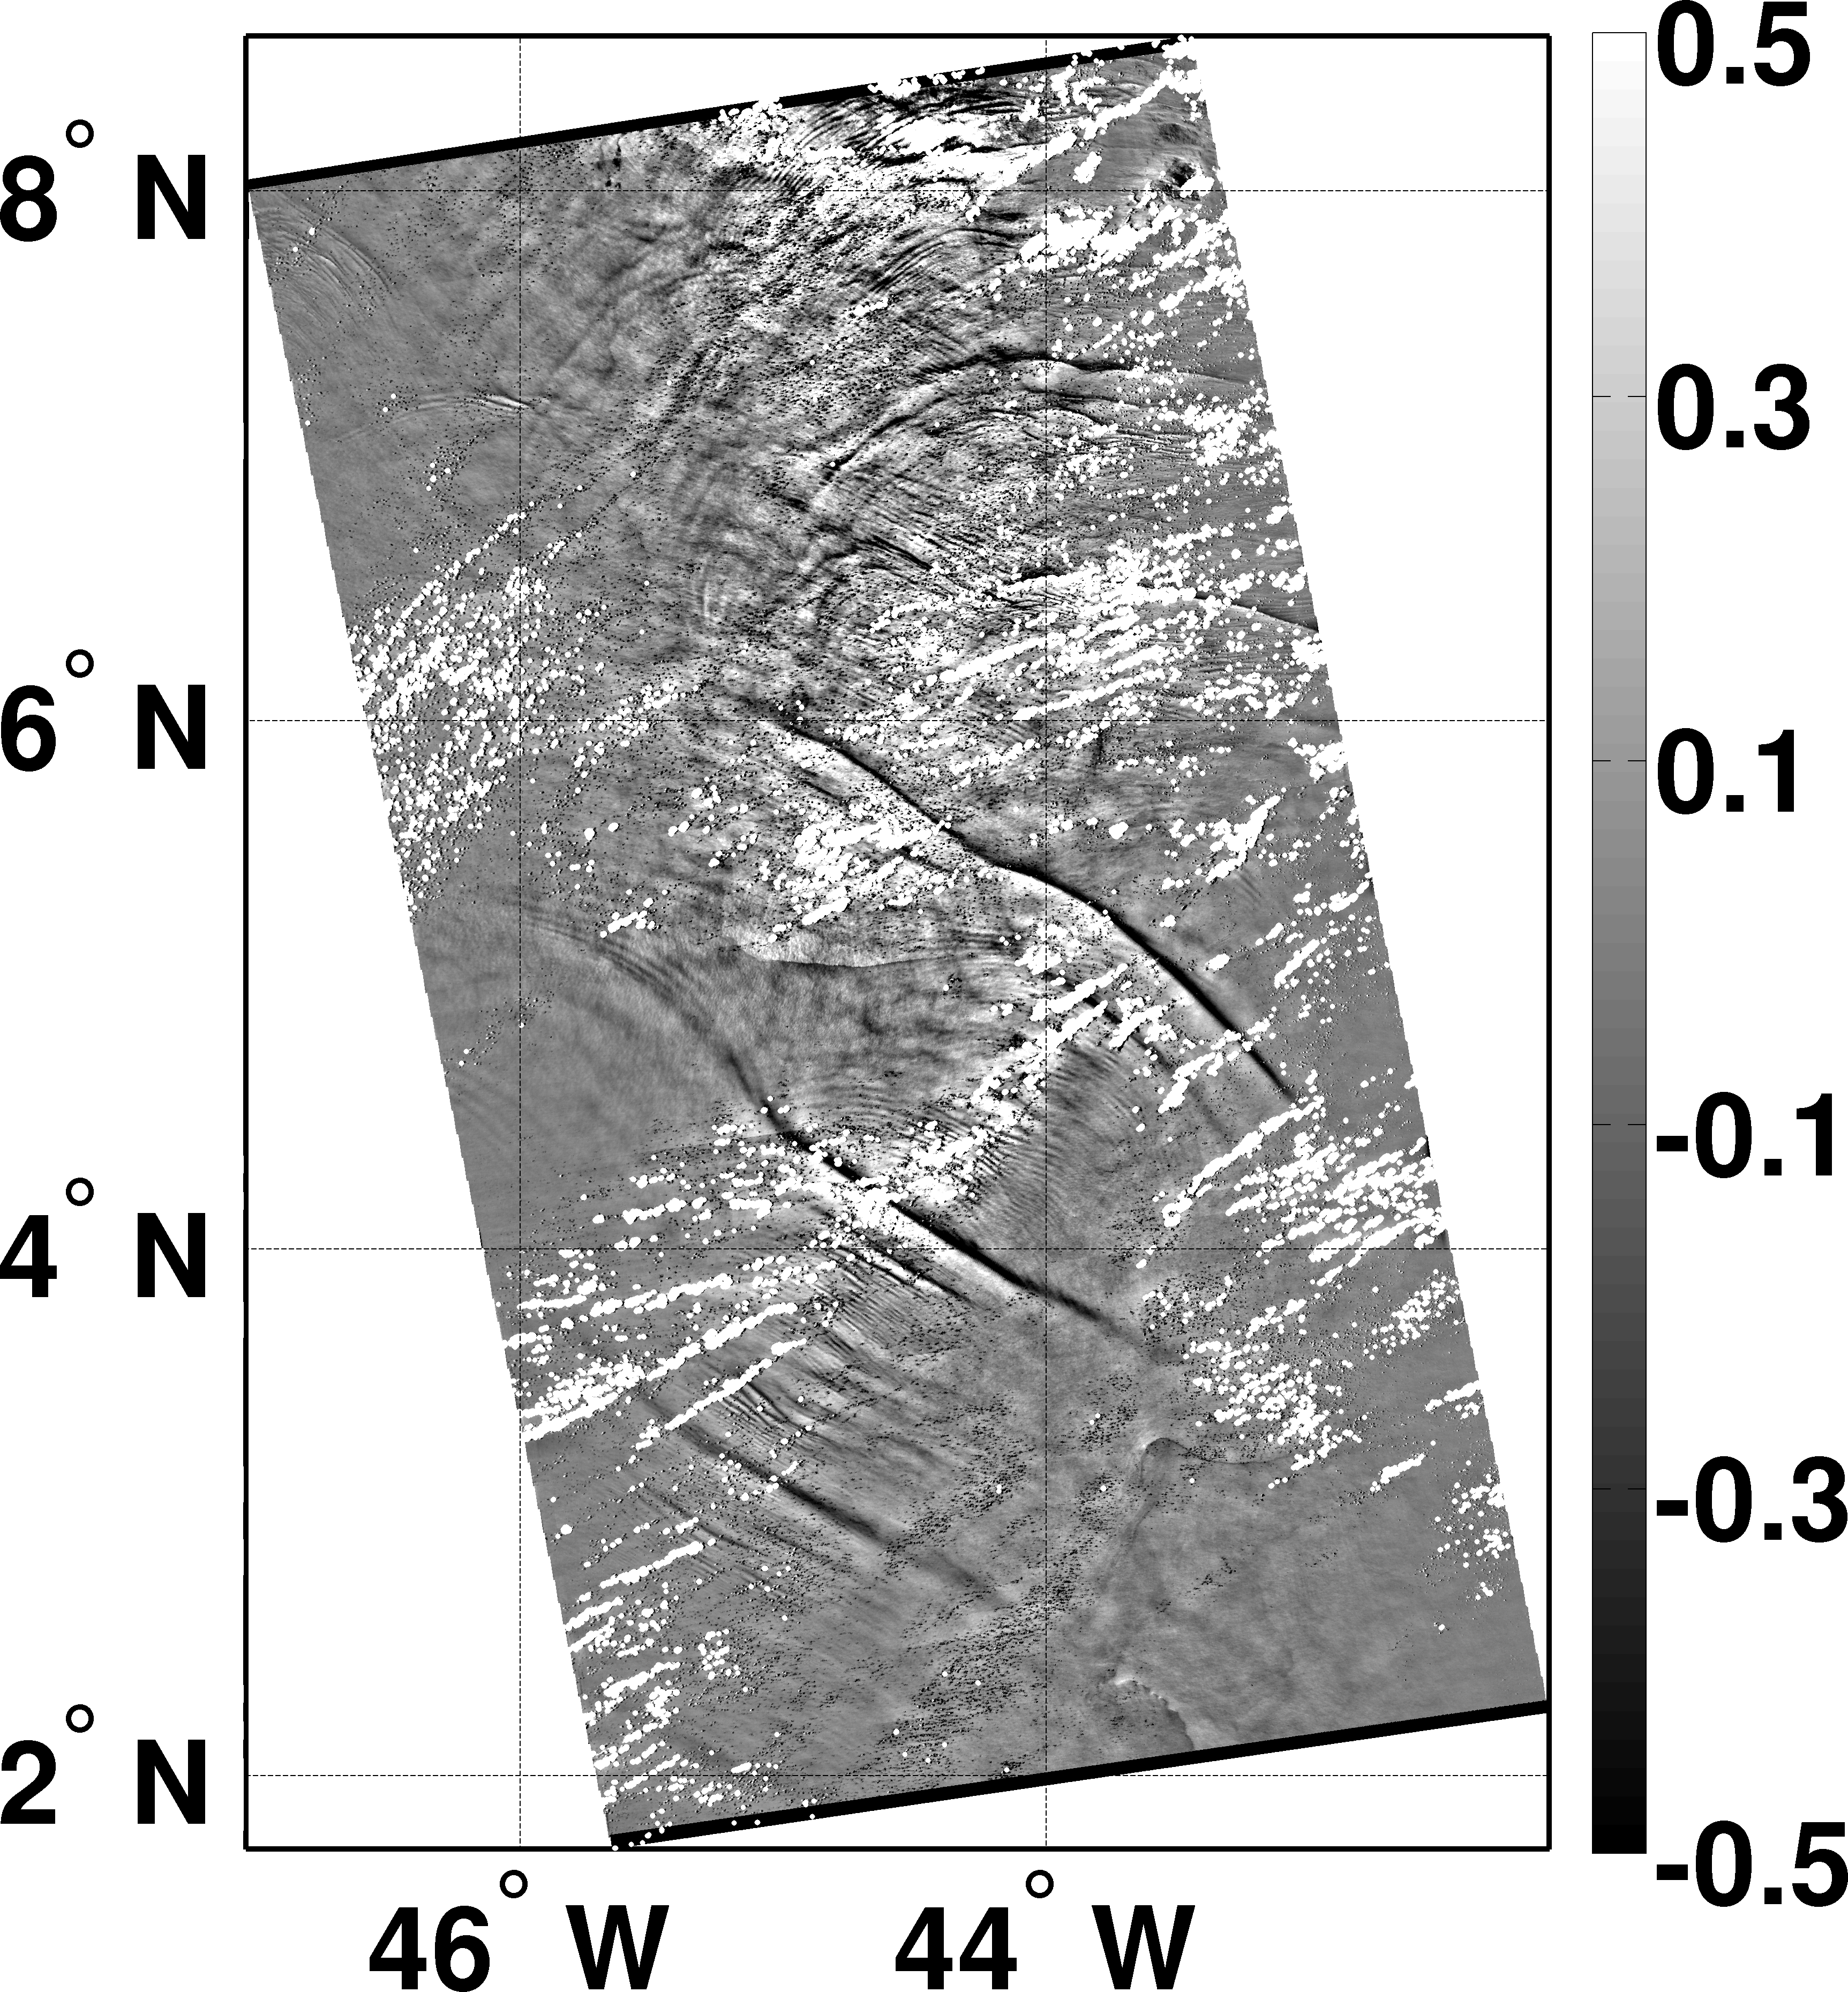
\includegraphics[width=20pc]{fig1b}
\\
\noindent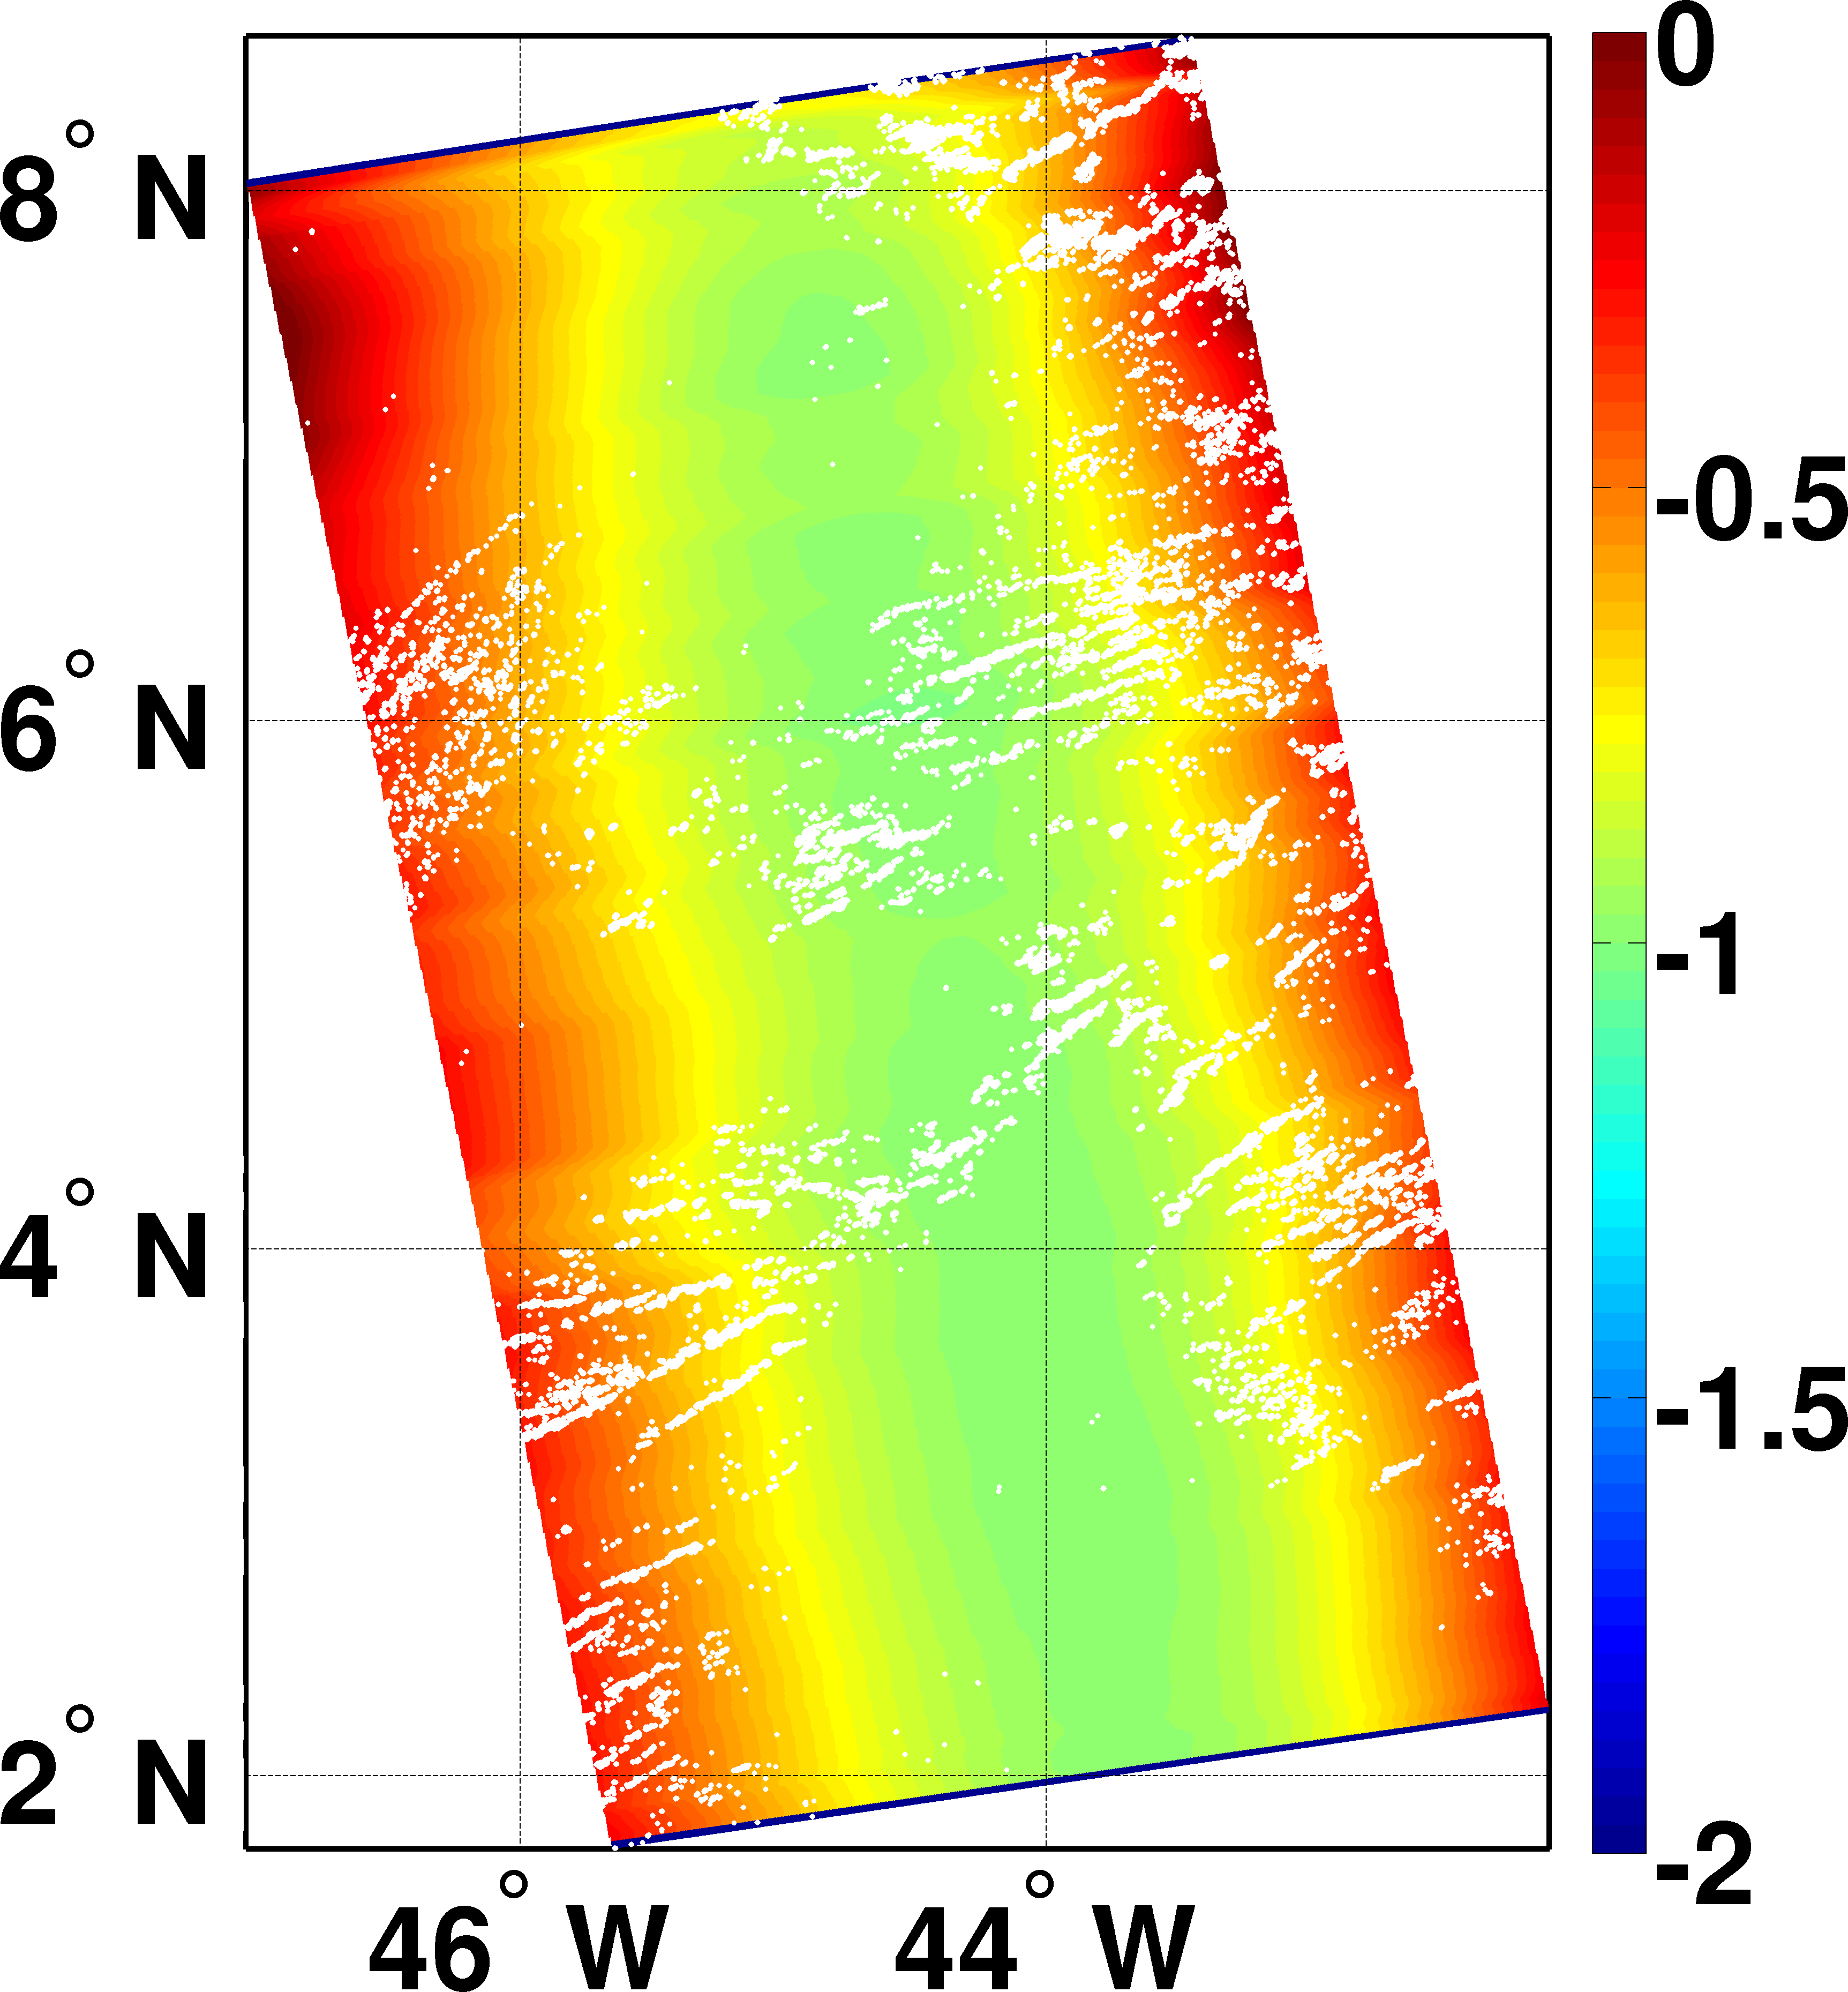
\includegraphics[width=20pc]{fig1c}
\hfill
\noindent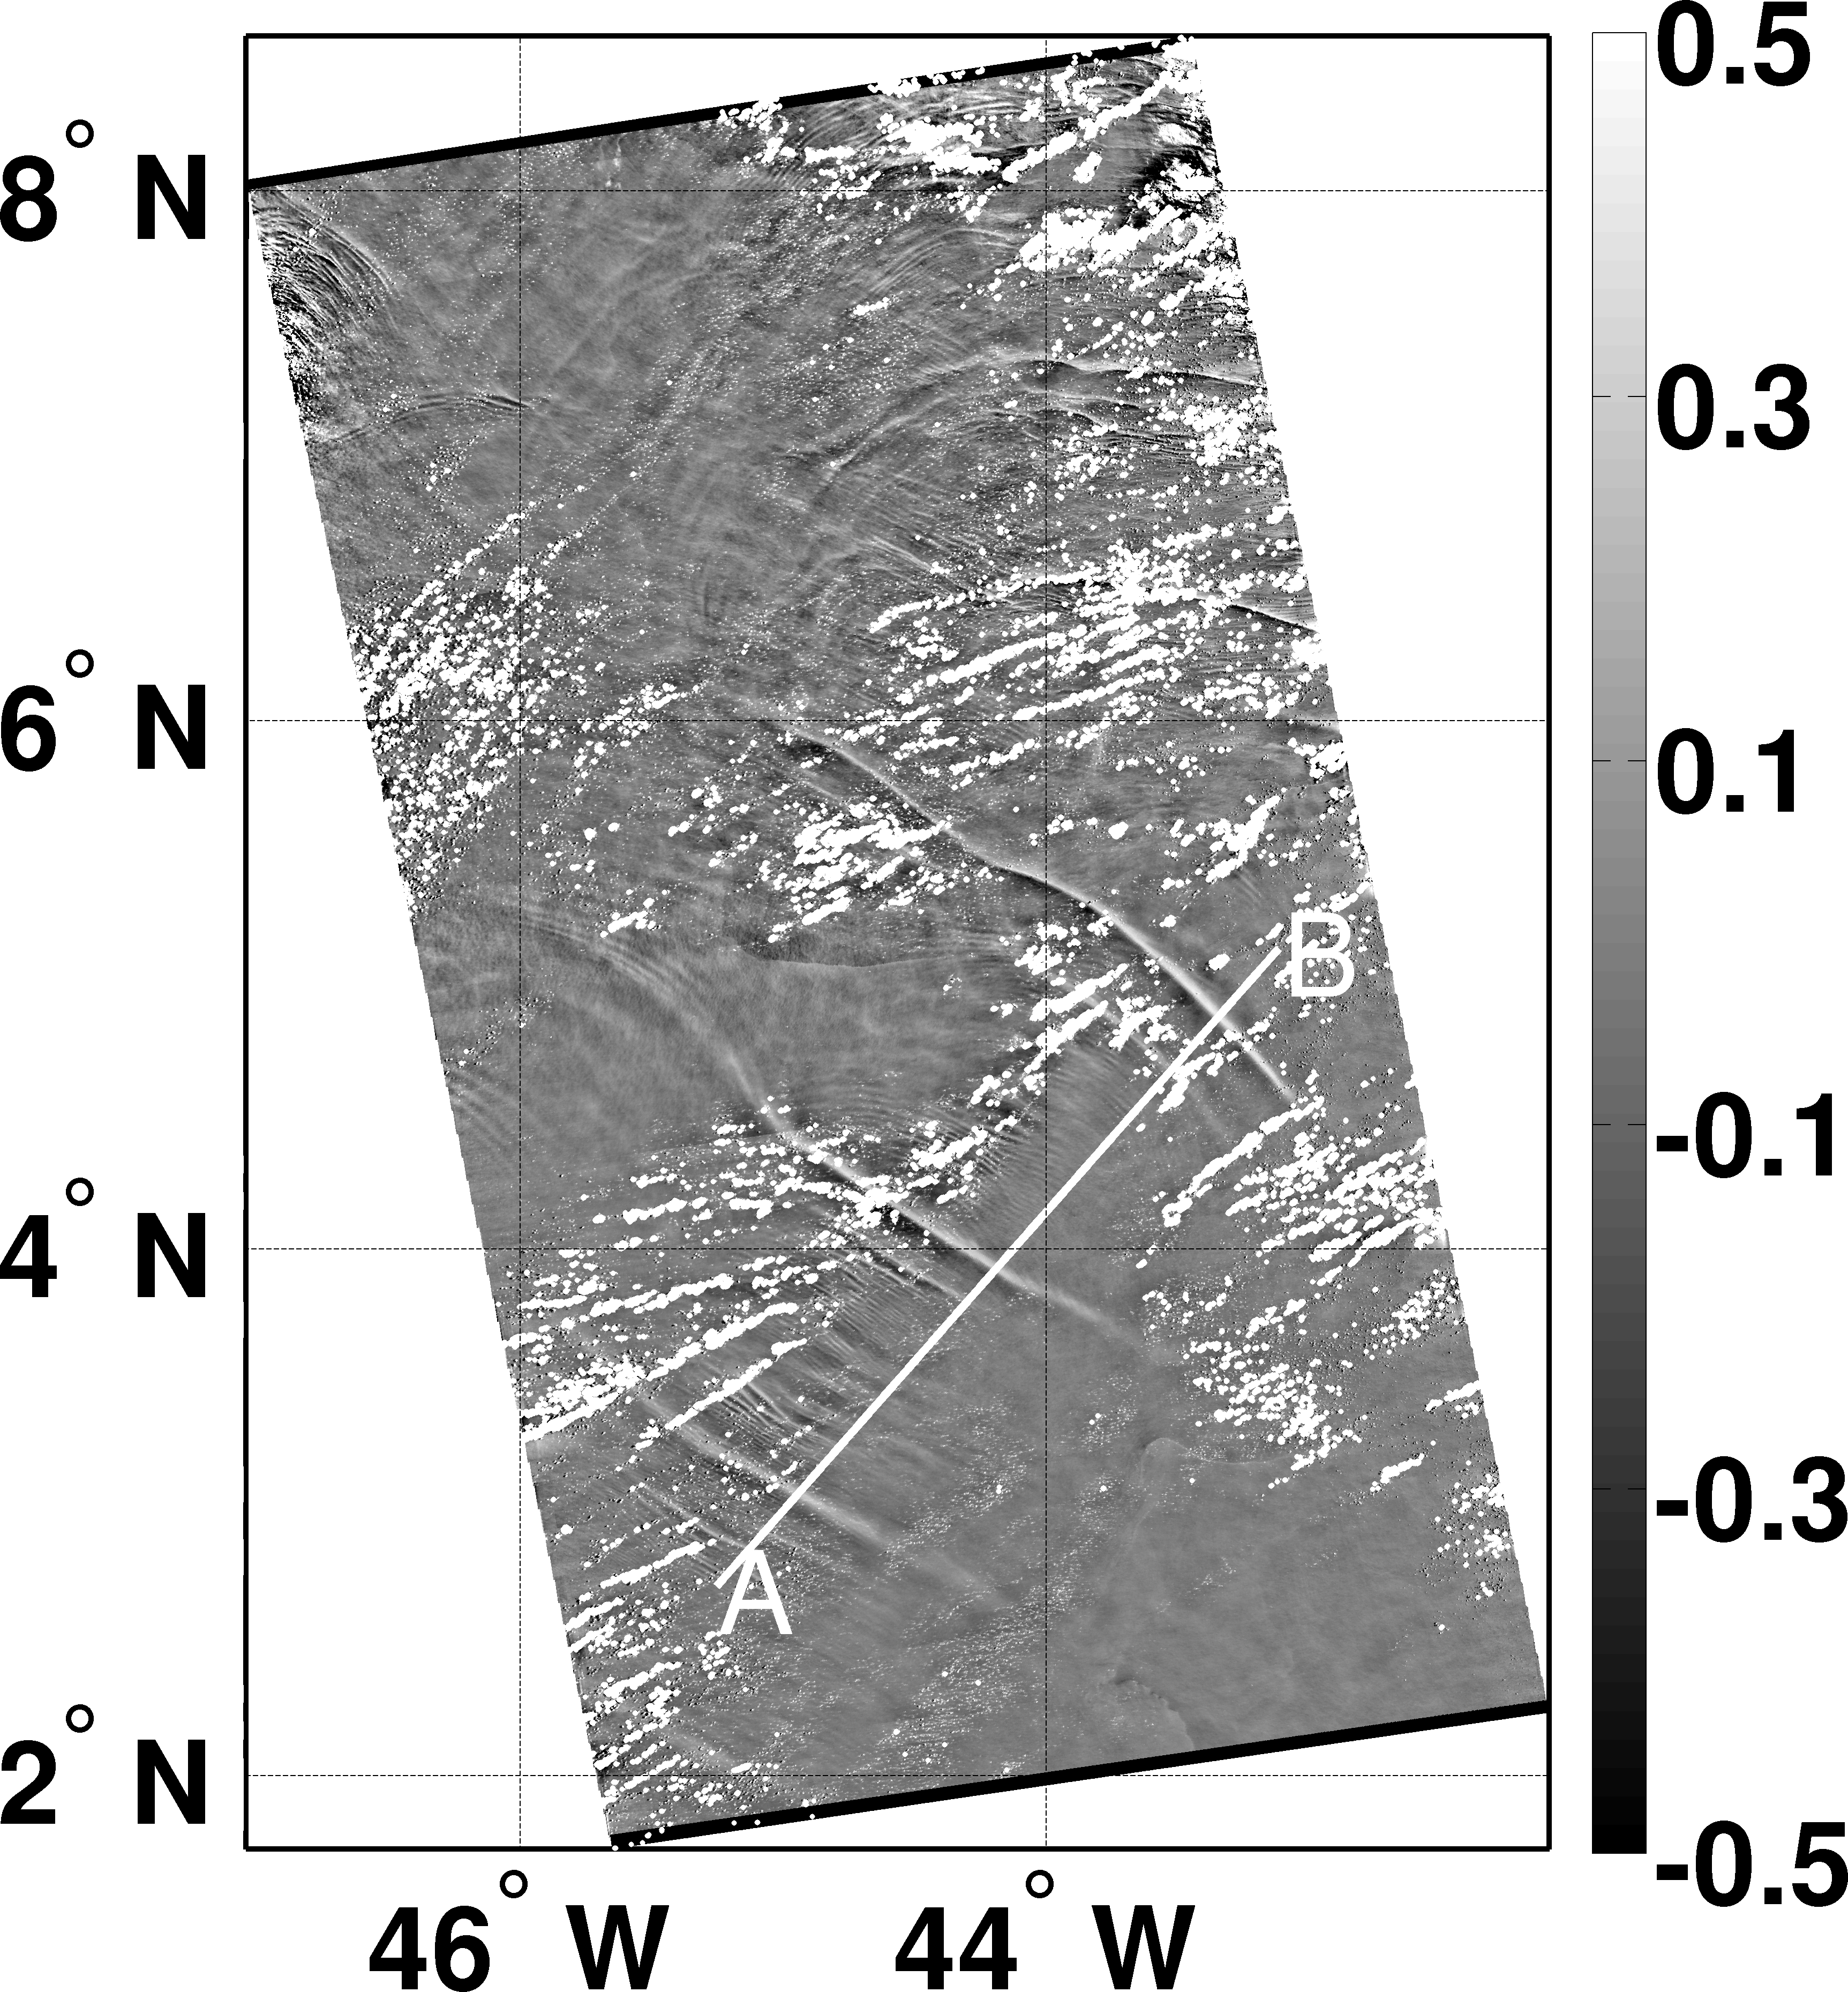
\includegraphics[width=20pc]{fig1d}
\caption{(upper left)  Fragment of the Aqua/MODIS image (April 26, 2009, 16:20) in red channel 850\textit{nm} of the Amazon Area containing IWs signatures. (upper right) Sunglint brightness variations $\tilde{B}$. (lower left) The transfer function $T$. (lower right) MSS variations retrieved from eq.(5) with (7) in \citep{Kudryavtsev2012a}. White areas are the clouds mask. Line A-B indicate location of the cross-section shown in Fig.~\ref{fig:2}.}
\label{fig:1}
\end{figure}


\begin{figure}
\noindent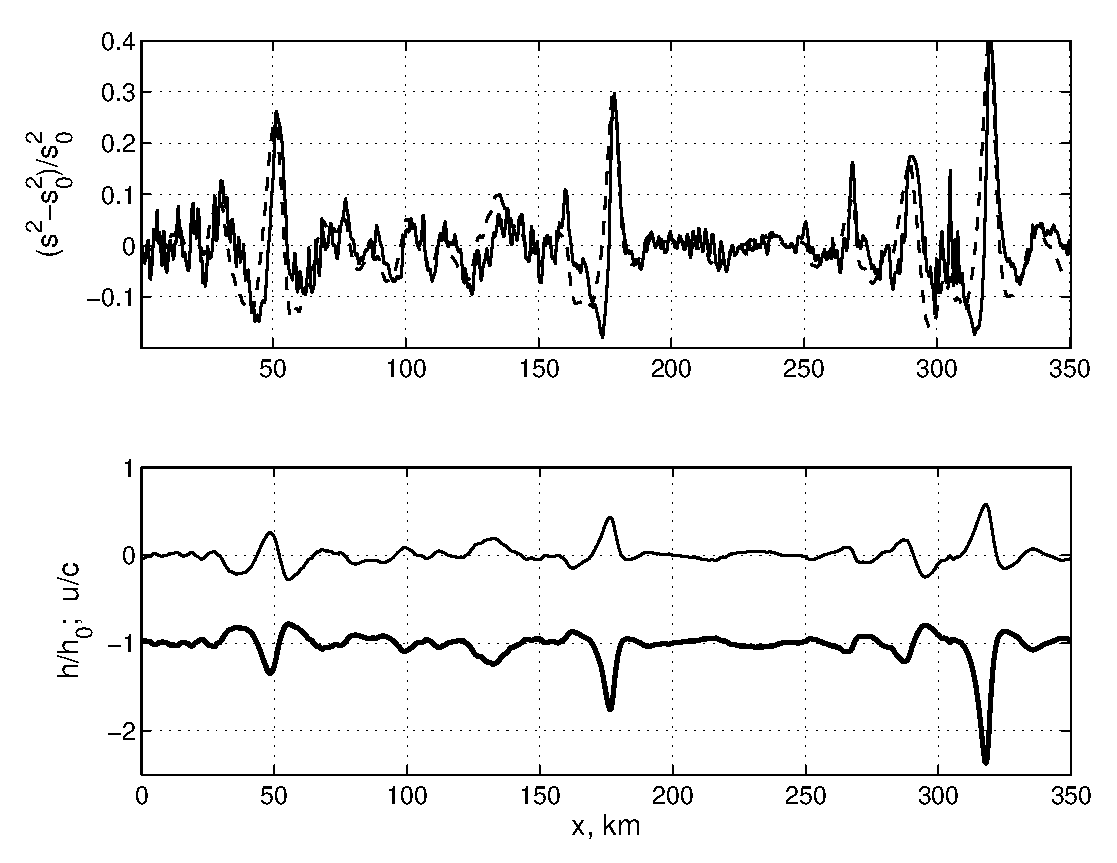
\includegraphics[width=\linewidth]{fig2.eps}
\caption{(upper) Profile of the MSS contrasts (solid line) along cross-sections A-B shown in Fig.~\ref{fig:1}. Dashed line shows RIM simulations. (lower) Displacement of the thermocline by IWs (thick line), and the current velocity induced by IWs on the surface (thin line).}
\label{fig:2}
\end{figure}

\end{document}